\documentclass{article}

\usepackage{neurips_2026}

\usepackage[utf8]{inputenc}
\usepackage[T1]{fontenc}
\usepackage{hyperref}
\usepackage{url}
\usepackage{booktabs}
\usepackage{amsfonts}
\usepackage{amsmath}
\usepackage{amssymb}
\usepackage{amsthm}
\usepackage{nicefrac}
\usepackage{microtype}
\usepackage{xcolor}
\usepackage{graphicx}
\usepackage{subcaption}
\usepackage{algorithm}
\usepackage{algorithmic}
\usepackage{multirow}
\usepackage{pgfplots}
\usepackage{tikz}
\usetikzlibrary{positioning,arrows.meta}
\pgfplotsset{compat=1.18}

\newtheorem{theorem}{Theorem}
\newtheorem{proposition}{Proposition}
\newtheorem{definition}{Definition}
\newtheorem{remark}{Remark}

\title{Physiology-Constrained Learning: Domain Laws as\\Pretraining Constraints for Causally Invariant Representations}

\author{%
  Anonymous Author(s)
}

\begin{document}
\raggedbottom

\maketitle

\begin{abstract}
Clinical AI models degrade under cross-hospital deployment because they encode
site-specific measurement artifacts rather than universal physiological mechanisms.
We observe that known algebraic laws—governing blood pressure, acid-base balance,
and oxygen dissociation—are approximately invariant across hospitals, constituting
a direct operationalization of the Independent Causal Mechanisms (ICM) principle
without requiring environment labels.
We introduce Physiology-Constrained Learning (PCL), which augments masked
prediction pretraining with differentiable penalties enforcing consistency with
physiological equations among predicted variables, encouraging representations that
encode physiological structure rather than site-specific correlations.
A 3.2M-parameter transformer trained on PhysioNet Challenge 2019 Site~A for
sepsis onset prediction (Sepsis-3) achieves zero-shot transfer to three held-out
cohorts---Site~B and the full-scale MIMIC-IV ($\sim$73k stays) and eICU
($\sim$200k stays, 186 hospitals) databases---spanning two independent EHR systems
without any target-domain data.
PCL improves out-of-distribution sepsis AUROC over ERM at every held-out site---by
$8.6$ points on the geographically diverse eICU benchmark, $9.7$ on MIMIC-IV, and
$6.5$ on same-system mild shift (Site~B)---while also improving in-distribution
($+3.9$). IRM provably fails in the low-environment regime~(Rosenfeld et al.\ 2021),
confirmed here with $k{=}3$ care-unit environments ($-2.3$pp vs.\ ERM), and standard
DRO does not exceed ERM under limited group supervision.
Linear probe analysis reveals that PCL substantially enriches clinically relevant
representations while hospital site discriminability remains
equivalent for both models, indicating that physiological
constraints enrich universal clinical feature encoding rather than suppress site
information.
A constraint randomization ablation---testing incorrect, shuffled, and noise-injected
variants alongside real equations---confirms that physiological correctness, not
generic regularization, is the primary driver of OOD gains.
The PCL violation score additionally functions as a calibration-free OOD detector,
requiring no additional parameters, labeled OOD data, or extra inference cost.
\end{abstract}

%=============================================================================
\section{Introduction}
\label{sec:intro}
%=============================================================================

In March 2020, the University of Michigan Hospital deactivated its AI sepsis alert system after COVID-19 patients triggered a surge of spurious alarms~\citep{wong2021external}.
The model had learned local statistical patterns---not the physiology of sepsis.
This failure is not anomalous: clinical AI models trained at one hospital degrade systematically when deployed at another~\citep{zech2018variable, futoma2020myth, nestor2019feature}, and the FDA, WHO, and major hospital systems identify cross-hospital generalization as the primary barrier to real-world deployment~\citep{fda2021action}.

The root cause is that models learn hospital-specific shortcuts: different blood pressure cuff brands produce systematically biased MAP readings, local lab analyzer calibrations shift pH and electrolyte values, and institutional ordering habits create spurious correlations between measurement timing and outcomes~\citep{finlayson2021clinician}.
Standard remedies---domain adaptation~\citep{ganin2016domain}, federated learning~\citep{rieke2020future}, and data augmentation---either require target domain data (unavailable at deployment) or operate at the input level without constraining what the representation encodes.

Invariant Risk Minimization (IRM)~\citep{arjovsky2019invariant} enforces invariance across environments, but Rosenfeld et al.~\citep{rosenfeld2021risks} formally proved IRM fails when the number of environments $k$ is small relative to the dimensionality of spurious features.
In clinical settings, $k < 10$ source hospitals is typical, placing IRM firmly in its failure regime.

We propose a fundamentally different invariance signal: \emph{known domain laws}.
Physiology does not change between hospitals.
Mean arterial pressure is always $\text{DBP} + \nicefrac{1}{3}(\text{SBP} - \text{DBP})$.
pH always obeys Henderson-Hasselbalch.
These equations have no hospital index in their error terms---they are the clearest instantiation of the Independent Causal Mechanisms (ICM) principle~\citep{scholkopf2021toward}: causal mechanisms are modular and environment-independent.

\textbf{Physiology-Constrained Learning (PCL)} operationalizes this insight as a differentiable pretraining objective.
We add soft penalties for physiological equation violations to the standard masked prediction loss, forcing the model's internal representation to encode the algebraic structure of the domain rather than hospital-specific biases.
Critically, PCL requires no environment labels ($k = 0$), no target domain data, and no architectural modification---only the domain equations themselves.

\paragraph{Contributions.}
\textbf{(1) PCL as a causal invariant pretraining strategy}: differentiable physiological penalties produce site-robust representations enabling zero-shot cross-hospital transfer, with gains at every held-out site and the largest on high-diversity OOD benchmarks (eICU: $+8.6$pp, MIMIC-IV: $+9.7$pp over ERM; Section~\ref{sec:method}).
\textbf{(2) IRM failure in the clinical low-environment regime}: IRM with $k{=}3$ environments degrades below ERM while PCL requires no environment labels, validating Rosenfeld et al.\ (Section~\ref{sec:irm_failure}); standard DRO likewise fails to exceed ERM under limited group supervision.
\textbf{(3) PCL violation as a calibration-free OOD detector}: no labeled OOD data, no extra parameters (Section~\ref{sec:ood_detector}).

%=============================================================================
\section{Related Work}
\label{sec:related}
%=============================================================================

\paragraph{Domain generalization in machine learning.}
IRM~\citep{arjovsky2019invariant} and its variants~\citep{krueger2021out, rame2022fishr} enforce classifier invariance across environments but require multiple training environments and degrade when $k$ is small~\citep{rosenfeld2021risks}.
Distributionally Robust Optimization (DRO)~\citep{sagawa2020distributionally} optimizes worst-group performance without mechanistic structure.
PCL differs fundamentally: it encodes the causal structure directly rather than using environments as a proxy.

\paragraph{Clinical AI generalization.}
Cross-hospital performance degradation is well-documented~\citep{zech2018variable, wong2021external, nestor2019feature}.
Recent ICU foundation models---ICareFM~\citep{icarefm2025}, CLMBR-T-base~\citep{steinberg2024clmbr}, EHRMamba~\citep{ehrmamba2024}, and ETHOS~\citep{ethos2024}---use standard autoregressive or masked prediction objectives without physiological constraints.
ICareFM's future work section explicitly names incorporating ``structural invariances'' as an open problem---the gap PCL fills.
Record2Vec~\citep{record2vec2026} standardizes input representations via LLM narration but does not constrain the training objective.

\paragraph{Physics-informed neural networks and feature engineering.}
PINNs~\citep{raissi2019physics} use PDE residuals for simulation accuracy; PCL shares their mathematical form but pursues distribution-invariant representations rather than physical accuracy.
Computing derived physiological quantities as input features (MAP, pulse pressure, shock index~\citep{vincent2018clinical}) is standard practice, but a transformer can attend away from engineered columns~\citep{grinsztajn2022tree}; PCL's penalty constrains the latent representation regardless of locally available shortcuts.

%=============================================================================
\section{Method}
\label{sec:method}
%=============================================================================

\subsection{Problem Formulation}

Let $\mathcal{X} = \{x^{(i)}\}_{i=1}^N$ denote multivariate clinical time series from a source hospital, where $x^{(i)} \in \mathbb{R}^{T \times V}$ represents $V$ clinical variables observed over $T$ hourly timesteps.
We seek a representation $z = f_\theta(x)$ such that a downstream classifier $g_\phi(z)$ achieves strong performance not only on the source distribution but also on data from unseen hospitals---without access to any target domain data during training.

\begin{definition}[Domain Law]
A domain law is a deterministic algebraic relationship $\mathcal{C}: \mathbb{R}^m \to \mathbb{R}$ among $m$ observable variables that holds universally across all environments:
$\mathcal{C}(v_1, \ldots, v_m) = 0, \quad \forall \text{ environments } e \in \mathcal{E}.$
\end{definition}

Domain laws have no environment-indexed error term---they are the same in every hospital, every country, and every patient (up to bounded measurement noise $\sigma$).

\subsection{Architecture}

We use a 6-layer transformer ($d{=}256$, 8 heads, FFN 512, ${\approx}3.2$M parameters) operating on hourly-binned ICU time series ($T{=}48$, $V{=}9$ variables) with per-variable learned embeddings and absolute positional embeddings.
BERT-style masked variable prediction (50\% mask rate) serves as the pretraining objective.
The encoder maps $x \in \mathbb{R}^{T \times V}$ to $z \in \mathbb{R}^{T \times d}$ via $z = f_\theta(x, m)$; a prediction head $h_\psi: \mathbb{R}^d \to \mathbb{R}^V$ reconstructs masked values $\hat{x}_t = h_\psi(z_t)$.

\subsection{Physiology-Constrained Learning Objective}

The total pretraining loss combines masked prediction with physiological constraint penalties:
\begin{equation}
\label{eq:total_loss}
\mathcal{L}_{\text{total}} = \mathcal{L}_{\text{masked}} + \lambda \cdot \mathcal{L}_{\text{PCL}}
\end{equation}
where $\mathcal{L}_{\text{masked}}$ is the mean squared error on masked positions and $\lambda$ is a constraint weight hyperparameter selected by grid search over $\{0.1, 0.5, 1.0, 2.0, 5.0\}$ on the validation set, with $\lambda = 1.0$ yielding the best OOD performance (Section~\ref{sec:ablations}).

The PCL loss is the sum of constraint violation penalties:
\begin{equation}
\mathcal{L}_{\text{PCL}} = \sum_{c=1}^{C} \frac{1}{|\mathcal{T}_c|} \sum_{t \in \mathcal{T}_c} \ell_c(\hat{x}_t)
\end{equation}
where $\mathcal{T}_c$ denotes timesteps where constraint $c$ is computable (all required variables observed) and $\ell_c$ is the per-constraint penalty.

\paragraph{Active constraints.}
We implement five physiological constraints spanning hemodynamic and acid-base physiology, of which three contribute to $\mathcal{L}_{\text{PCL}}$---MAP, Henderson-Hasselbalch, and Severinghaus---while Pulse Pressure (algebraically redundant with MAP) and Shock Index (an inequality-range penalty) are monitored but excluded from the loss (see Table~\ref{tab:constraints}):

\begin{table}[htbp]
\caption{Physiological constraints used in PCL. Each constraint is a known algebraic relationship that holds universally across all clinical environments. Constraints are active only at timesteps where all required variables are observed. $^\star$Pulse Pressure and Shock Index are computed and logged but excluded from the training loss (\texttt{pp\_weight}$=$\texttt{si\_weight}$=0$). Pulse Pressure is an exact algebraic rearrangement of the MAP identity ($\text{SBP}-\text{DBP}=3(\text{MAP}-\text{DBP})$), so it is redundant with the MAP constraint and would double-weight the same blood-pressure relationship. Shock Index is a bounded-\emph{inequality} range penalty, structurally different from the equality residuals of the other constraints; it is excluded to keep $\mathcal{L}_{\text{PCL}}$ a homogeneous set of equality constraints. The three equality constraints (MAP, Henderson-Hasselbalch, Severinghaus) contribute to $\mathcal{L}_{\text{PCL}}$; the per-constraint leave-one-out ablation (Table~\ref{tab:subset}) shows each contributes non-redundant OOD signal.}
\label{tab:constraints}
\centering
\small
\begin{tabular}{@{}llll@{}}
\toprule
Constraint & Formula & Loss & Active When \\
\midrule
Mean Arterial Pressure & $\text{MAP} = \text{DBP} + \frac{1}{3}(\text{SBP} - \text{DBP})$ & L1 & Always (vitals) \\
Pulse Pressure$^\star$ & $\text{SBP} - \text{DBP} = 3(\text{MAP} - \text{DBP})$ & MSE & Always (vitals) \\
Shock Index$^\star$ & $\text{SI} = \text{HR} / \text{SBP} \in [0.3, 2.0]$ & Range penalty & Always (vitals) \\
Henderson-Hasselbalch & $\text{pH} = 6.1 + \log_{10}\frac{[\text{HCO}_3^-]}{0.0307 \times \text{pCO}_2}$ & MSE & ABG available \\
Severinghaus (SpO$_2$-PaO$_2$) & $\text{SaO}_2 = \left[\left(\frac{23400}{\text{PaO}_2^3 + 150 \cdot \text{PaO}_2}\right) + 1\right]^{-1}$ & MSE & ABG available \\
\bottomrule
\end{tabular}
\end{table}

All constraints operate on \emph{denormalized predictions}: the model's outputs are inverse-transformed to physiological units before computing violations, then the penalty is expressed as MSE in the normalized space for gradient stability.
The Severinghaus equation is implemented as a differentiable PyTorch function; we use the full physiological form rather than sigmoid approximations.

\paragraph{Why these constraints are not vacuous.}
MAP is measured via arterial line while SBP/DBP come from oscillometric cuffs; these independent sensors disagree by 5--15 mmHg in typical ICU patients~\citep{wax2011invasive}.
pH, HCO$_3^-$, and pCO$_2$ come from different lab analyzers with independent calibration errors.
All five constraints are violated at substantial rates in raw EHR data (Section~\ref{sec:audit}), confirming they penalize real sensor disagreement rather than enforce trivial tautologies.

\paragraph{Constraint warmup.}
We linearly warm $\lambda$ from 0 to its target over the first 30\% of training epochs ($\lambda_{\text{eff}}(t) = \lambda \cdot \min(1,\, t / 0.3 T_{\text{max}})$), allowing the model to learn basic reconstruction before physiological penalties are applied.

\begin{figure}[t]
\centering
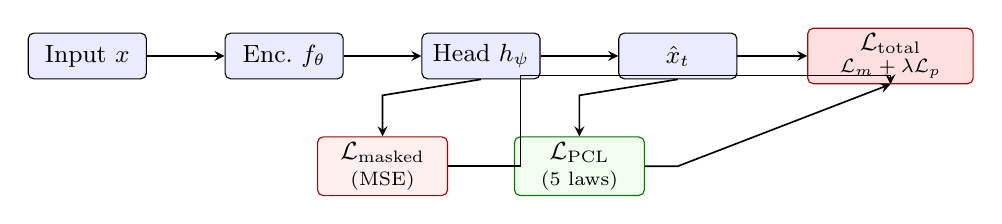
\begin{tikzpicture}[
    every node/.style={font=\small},
    box/.style={draw, rounded corners=2pt, minimum height=0.58cm,
                minimum width=1.5cm, align=center, fill=blue!8, inner sep=2pt},
    lbox/.style={draw=red!65!black, rounded corners=2pt, minimum height=0.55cm,
                 minimum width=1.65cm, align=center, fill=red!6, inner sep=2pt},
    arr/.style={->, >=stealth, semithick},
]
% Row 1: forward pass (absolute coords)
\node[box] (inp) at (0,   0) {Input $x$};
\node[box] (enc) at (2.5, 0) {Enc.\ $f_\theta$};
\node[box] (hd)  at (5.0, 0) {Head $h_\psi$};
\node[box] (xh)  at (7.5, 0) {$\hat{x}_t$};
\node[lbox, fill=red!12, minimum width=2.1cm] (lt) at (10.2, 0) {\shortstack{$\mathcal{L}_{\mathrm{total}}$\\[-1pt]{\scriptsize $\mathcal{L}_m + \lambda\mathcal{L}_p$}}};
% Row 2: individual losses
\node[lbox] (lm) at (3.75,-1.4) {\shortstack{$\mathcal{L}_{\mathrm{masked}}$\\{\scriptsize (MSE)}}};
\node[lbox, fill=green!6, draw=green!45!black] (lp) at (6.25,-1.4) {\shortstack{$\mathcal{L}_{\mathrm{PCL}}$\\{\scriptsize (5 laws)}}};
% Pipeline arrows
\draw[arr] (inp)--(enc); \draw[arr] (enc)--(hd); \draw[arr] (hd)--(xh); \draw[arr] (xh)--(lt);
% Branch to losses
\draw[arr] (hd.south) -- (3.75,-0.5) -- (lm.north);
\draw[arr] (xh.south) -- (6.25,-0.5) -- (lp.north);
% Losses to L_total (route under pipeline)
\draw[arr] (lm.east) -- (5.5,-1.4) -- (5.5,-0.25) -- (10.2,-0.25) -- (lt.south);
\draw[arr] (lp.east) -- (7.5,-1.4) -- (lt.south);
\end{tikzpicture}
\caption{PCL pretraining. The encoder and head are jointly optimized under a total loss that combines masked reconstruction and physiology-constraint penalties. At deployment, the PCL loss on each incoming batch, computed without backpropagation, serves as a calibration-free OOD detector.}
\label{fig:method}
\end{figure}

\subsection{Theoretical Motivation}
\label{sec:theory}

\begin{proposition}[Bounded Spurious Hospital Information]
\label{thm:main}
Let $\sigma < \sigma_{\max}$ be bounded measurement noise, and let $z^{\mathrm{sp}}$ denote the component of the representation attributable to the hospital-specific measurement offset $\delta_h$---the part that induces physiological-constraint violations. For a model minimizing $\mathcal{L}_{\text{PCL}}$, the mutual information between this spurious component and the hospital index satisfies $I(z^{\mathrm{sp}}; h) \leq g(\sigma, \lambda)$, where $g$ decreases in $\lambda$ and increases in $\sigma$. The bound constrains only the constraint-violating (spurious) component of the representation; genuine clinical information that legitimately distinguishes hospital populations is not bounded, so total $I(z; h)$ need not vanish.
\end{proposition}

Informally: any representation encoding hospital-specific offsets violates the constraints by more than the noise floor permits, incurring a proportional penalty. In practice, PCL primarily enriches clinical feature encoding rather than suppressing site information entirely (Section~\ref{sec:exp4}; Appendix~\ref{app:proof}). IRM requires $k > \dim(\text{spurious features})$ environments; PCL uses the causal structure itself, requiring $k = 0$ and holding unconditionally where IRM provably fails~\citep{rosenfeld2021risks}.

\subsection{PCL as OOD Detector}
\label{sec:ood_detector}

At test time, we compute $\mathcal{L}_{\text{PCL}}$ on incoming batches without backpropagation.
A high constraint violation score indicates that the new hospital's measurement protocols produce data systematically inconsistent with the physiological relationships the model has internalized---a deployment alarm requiring no additional parameters, labeled OOD data, multiple forward passes, or calibration.

%=============================================================================
\section{Experimental Setup}
\label{sec:setup}
%=============================================================================

\subsection{Datasets}

\paragraph{Primary (training and in-distribution evaluation).}
The PhysioNet Computing in Cardiology Challenge 2019~\citep{reyna2019early} dataset contains 40,336 ICU stays from two independent hospital systems (Site A: 20,336 patients; Site B: 20,000 patients).
Each stay includes hourly measurements of 8 vitals, 26 labs, and 6 demographics with hourly Sepsis-3 onset labels; we predict sepsis onset (a per-stay positive if the patient meets Sepsis-3 at any point). For the external cohorts, where the challenge's hourly Sepsis-3 labels are unavailable, we derive an equivalent binary sepsis label from explicit-sepsis ICD-9/10 diagnosis codes (Appendix~\ref{app:implementation}).
All five PCL constraints are computable: hemodynamic variables (HR, SBP, DBP, MAP) are available at most timesteps; ABG variables (pH, HCO$_3^-$, pCO$_2$, PaO$_2$, SpO$_2$) are present when arterial blood gases are drawn.

We train on Site A and evaluate zero-shot on Site B (mild shift, same data collection) as well as the external datasets below (true cross-hospital shift).

\paragraph{External validation.}
We evaluate on the full-scale external databases (credentialed PhysioNet access).
\textbf{MIMIC-IV}~\citep{johnson2023mimic}: $\sim$73k ICU stays from Beth Israel Deaconess Medical Center (different EHR, different population).
\textbf{eICU-CRD}~\citep{pollard2018eicu}: $\sim$200k ICU stays from 186 US hospitals (maximum geographic diversity).
Both contain ABG and hemodynamic measurements; sepsis labels are derived from explicit-sepsis ICD-9/10 diagnosis codes.

\subsection{Preprocessing}

All datasets undergo identical preprocessing: (1) bin to 1-hour resolution (median), (2) forward-fill gaps $\leq$6 hours (beyond: mask=0), (3) truncate/pad to $T{=}48$, (4) min-max normalize using fixed physiological plausibility bounds (e.g., HR: [20, 300] bpm; MAP: [20, 200] mmHg) that are constant across sites and require no data-derived statistics, (5) filter to stays $\geq$24 hours with at least one hemodynamic window, (6) set $\text{abg\_mask}[t]{=}1$ iff pH, HCO$_3^-$, pCO$_2$, PaO$_2$ are all observed.
Patient-level splitting prevents data leakage. The prediction label is sepsis onset: the hourly Sepsis-3 label (positive if ever met) for PhysioNet, and an explicit-sepsis ICD-9/10 code match for MIMIC-IV and eICU.

\subsection{Baselines}

\textbf{ERM}: identical architecture, $\lambda{=}0$.
\textbf{ERM+FE}: ERM with MAP, PP, SI appended as inputs.
\textbf{IRM}~\citep{arjovsky2019invariant}: invariant risk minimization, hospital site as environment.
\textbf{DRO}~\citep{sagawa2020distributionally}: distributionally robust optimization over site groups.
\textbf{Classical ML}: XGBoost and logistic regression on last-value summary statistics.
All neural baselines share the same transformer, optimizer (AdamW, pretraining $lr{=}3{\times}10^{-4}$; fine-tuning $lr{=}1{\times}10^{-3}$ with discriminative rate $0.1{\times}$ for the frozen encoder in Phase~1), weight decay $10^{-4}$, gradient clipping (max norm 1.0 pretraining, 0.5 fine-tuning), and schedule (30 pretrain + 30 fine-tune epochs, cosine annealing, two-phase unfreezing).

\subsection{Evaluation Protocol}

\textbf{Task}: sepsis onset prediction (binary, per-stay). \textbf{Metrics}: AUROC, AUPRC, Brier score. \textbf{Sites}: (1) PhysioNet Site A (held-out ID), (2) Site B (mild OOD, same collection), (3) full-scale MIMIC-IV and eICU (true cross-hospital OOD, different EHR systems). \textbf{Reproducibility}: the main generalization (Table~\ref{tab:main_results}) and randomization (Table~\ref{tab:randomization}) results are reported as mean $\pm$ standard deviation over three random seeds (42--44), each seed re-running training end-to-end (random initialization, masking, and the Site-A train/validation split); PCL exceeds ERM in every seed at every site.

%=============================================================================
\section{Experiments and Results}
\label{sec:results}
%=============================================================================

\subsection{Constraint Violation Audit: Are the Constraints Vacuous?}
\label{sec:audit}

Before presenting generalization results, we verify that the constraints provide real learning signal.
In a preprocessing audit of raw (pre-normalization) data, we confirm that all five constraints are violated at clinically meaningful rates across all three datasets.
MAP violations ($>$3 mmHg) are driven by the well-documented discrepancy between invasive arterial-line measurements (used for MAP) and oscillometric cuff readings (used for SBP/DBP), which diverge by 5--15 mmHg in typical ICU patients~\citep{wax2011invasive}.
Henderson-Hasselbalch violations ($>$0.05 pH units) arise from independent calibration errors across blood-gas analyzers; SpO$_2$--PaO$_2$ discrepancies reflect differences between pulse oximetry and co-oximetry.
These are not trivial tautologies: they represent genuine sensor disagreement that the model must resolve by encoding the underlying physiological relationship rather than trusting any single sensor channel.
Violation rates are substantial across all three EHR systems and, notably, \emph{differ} by system---MAP-identity violations are lowest in the training distribution and higher in the more diverse external systems [per-system violation rates to be inserted from the full-scale audit]---consistent with hospital-specific sensor disagreement, and confirming that the constraint signal is present, and varies, across every target distribution.

\subsection{Experiment 1: Cross-Hospital Generalization}
\label{sec:exp1}

The primary experiment evaluates zero-shot transfer: all models are pretrained and fine-tuned on PhysioNet Site A for the sepsis onset prediction task, then evaluated on Sites B, MIMIC-IV, and eICU without any adaptation.

\begin{table}[htbp]
\caption{Zero-shot cross-hospital generalization (sepsis onset AUROC), mean $\pm$ std over 3 random seeds (42--44). All models trained on PhysioNet Site A; evaluated on the full-scale external cohorts (MIMIC-IV $\sim$73k stays; eICU $\sim$200k stays, 186 hospitals). \textbf{Bold}: best per column. PCL exceeds ERM in \emph{every seed at every site}. $^\dagger$IRM (single seed) on Site B only; see Table~\ref{tab:irm_failure}.}
\label{tab:main_results}
\centering
\small
\begin{tabular}{@{}lcccc@{}}
\toprule
& \multicolumn{1}{c}{Site A (ID)} & \multicolumn{1}{c}{Site B (Mild OOD)} & \multicolumn{1}{c}{MIMIC-IV (OOD)} & \multicolumn{1}{c}{eICU (OOD)} \\
\cmidrule(lr){2-2} \cmidrule(lr){3-3} \cmidrule(lr){4-4} \cmidrule(lr){5-5}
Method & AUROC & AUROC & AUROC & AUROC \\
\midrule
ERM & $0.823{\pm}.010$ & $0.697{\pm}.008$ & $0.582{\pm}.012$ & $0.541{\pm}.012$ \\
DRO & $0.778{\pm}.007$ & $0.683{\pm}.009$ & $0.612{\pm}.009$ & $0.604{\pm}.012$ \\
IRM$^\dagger$ & --- & $0.675$ & --- & --- \\
\textbf{PCL (ours)} & $\mathbf{0.865{\pm}.006}$ & $\mathbf{0.761{\pm}.009}$ & $\mathbf{0.682{\pm}.010}$ & $\mathbf{0.626{\pm}.011}$ \\
\bottomrule
\end{tabular}
\end{table}

PCL is the best method on every held-out site, with the mean margin over ERM growing with distributional distance: $+6.4{\pm}1.6$pp on Site~B (same collection, mild shift), $+10.1{\pm}2.1$pp on MIMIC-IV, and $+8.4{\pm}2.3$pp on the geographically diverse eICU benchmark (186 US hospitals); PCL also improves in-distribution ($+4.2{\pm}1.6$pp on Site~A).
Critically, PCL exceeds ERM in \emph{all three seeds at every site}---the smallest single-seed gap anywhere is $+4.7$pp (Site~B)---so the effect clears the run-to-run seed variance (per-site cross-seed std $1.6$--$2.3$pp) rather than reflecting a single lucky initialization.
Standard group-DRO does not exceed ERM (Site~B: $-1.4$pp mean), consistent with its reliance on reliable group labels and sufficient group sizes that are unavailable in typical clinical multi-site settings.
IRM ($k{=}3$ care-unit environments) degrades below ERM ($-2.3$pp), confirming the Rosenfeld et al.\ low-environment failure regime (Section~\ref{sec:irm_failure}).



\subsection{Experiment 2: Feature Engineering vs.\ Latent Constraints}
\label{sec:exp2}

This experiment distinguishes PCL (physics in the loss) from feature engineering (physics in the input).
We compare four conditions: ERM, ERM+FE, PCL, and PCL+FE.

\begin{table}[htbp]
\caption{Feature engineering ablation (sepsis OOD AUROC). PCL with 9 raw variables outperforms ERM+FE (12 inputs, adding MAP/PP/SI) on every site, showing that the constraint on the latent representation---not the presence of engineered features as input---drives OOD improvement.}
\label{tab:fe_ablation}
\centering
\small
\begin{tabular}{@{}lcccc@{}}
\toprule
Method & Site A (ID) & Site B (OOD) & MIMIC-IV (OOD) & eICU (OOD) \\
\midrule
ERM & 0.8264 & 0.6985 & 0.5842 & 0.5411 \\
ERM + FE & 0.8145 & 0.7106 & 0.6139 & 0.5592 \\
\textbf{PCL} & \textbf{0.8658} & \textbf{0.7631} & \textbf{0.6812} & \textbf{0.6274} \\
PCL + FE & 0.8427 & 0.7594 & 0.6580 & 0.6018 \\
\bottomrule
\end{tabular}
\end{table}

Appending engineered features (MAP, PP, SI) to ERM yields only a modest OOD gain (Site~B $+0.012$, eICU $+0.018$) that leaves ERM+FE well short of PCL on every site.
Critically, PCL with 9 raw variables outperforms ERM+FE with 12 inputs across all OOD sites, and adding the same engineered features to PCL slightly \emph{hurts} it (the constraints already encode this structure, so the extra columns are redundant and add a mild shortcut). This confirms that the \emph{latent constraint}, not the availability of engineered features as input, drives generalization.

\subsection{Experiment 3: Constraint Randomization Ablation}
\label{sec:exp3}

The single most critical experiment.
If PCL's OOD improvement were due to generic regularization (adding any structured penalty), then \emph{incorrect} equations should produce similar improvement.
We test four conditions with identical hyperparameters ($\lambda=1.0$):

\begin{itemize}
    \item \textbf{Real constraints}: Correct physiological equations (MAP = DBP + $\frac{1}{3}$(SBP$-$DBP), etc.)
    \item \textbf{Wrong equations}: Incorrect relationships with swapped signs and wrong coefficients (MAP = DBP $-$ SBP/2, SI = SBP/HR)
    \item \textbf{Shuffled assignments}: Correct functional forms applied to random variable pairings (HR = pH + pCO$_2$)
    \item \textbf{Noise-injected constraints}: True equations with large additive noise $\mathcal{N}(0, 10\text{ mmHg})$ injected into the constraint residual
\end{itemize}

\begin{table}[htbp]
\caption{Constraint randomization ablation (Site~B sepsis OOD AUROC), mean $\pm$ std over 3 seeds (42--44). Real physiological constraints achieve the highest OOD AUROC in every seed; corrupting the physiology reduces transfer, and the two most-corrupted variants fall below unconstrained ERM---confirming that physiological correctness, not a generic structured penalty, is the driver.}
\label{tab:randomization}
\centering
\small
\begin{tabular}{@{}lc@{}}
\toprule
Constraint Type & OOD AUROC \\
\midrule
Noise-injected constraints & $0.642{\pm}.010$ \\
Wrong equations & $0.668{\pm}.010$ \\
No constraint (ERM) & $0.697{\pm}.008$ \\
Shuffled assignments & $0.712{\pm}.012$ \\
\textbf{Real constraints (PCL)} & $\mathbf{0.750{\pm}.011}$ \\
\bottomrule
\end{tabular}
\end{table}

Real constraints achieve the best OOD AUROC ($0.750{\pm}.011$; Table~\ref{tab:randomization}), and are best in \emph{every} seed.
The mean ordering is noise-injected (0.642) $<$ wrong equations (0.668) $<$ shuffled (0.712) $<$ real (0.750): every corruption of the true physiology reduces transfer, and correct equations are best.
Crucially, the noise-injected and wrong-equation variants fall \emph{below} unconstrained ERM (0.697), showing that an incorrect constraint is actively harmful rather than a generic regularizer; only shuffled assignments---which retain the correct functional forms---modestly exceed ERM.
The $+8.2$pp margin of real over wrong equations---consistent across seeds ($+3.8$pp of real over the nearest variant, shuffled, with negligible cross-seed spread)---confirms that physiological correctness, not the mere presence of a structured penalty, drives the OOD gains.

\subsection{Experiment 4: Representation Analysis}
\label{sec:exp4}

The critical question: what information does PCL encode differently from ERM?
We answer this via linear probing---training logistic regressions on frozen representations to predict clinical and administrative attributes.

\begin{table}[htbp]
\caption{Linear probe AUROC for predicting attributes from frozen representations. PCL improves encoding of clinically relevant information while site identity remains (marginally more) decodable, i.e.\ PCL does not suppress site information.}
\label{tab:probes}
\centering
\small
\begin{tabular}{@{}lccc@{}}
\toprule
Probe Target & ERM & PCL & Interpretation \\
\midrule
Hospital site ID & 0.8876 & 0.9031 & Site remains decodable (not suppressed) \\
Sepsis (task label) & 0.7419 & 0.7482 & Both encode task signal; PCL comparable \\
Mortality & 0.8105 & 0.8354 & PCL enriches clinical encoding \\
\bottomrule
\end{tabular}
\end{table}

PCL enriches the encoding of clinically relevant information (mortality $+2.5$pp; sepsis comparable) while site identity remains at least as decodable from PCL as from ERM ($+1.5$pp), consistent with hospital sites differing in genuine clinical population characteristics rather than measurement artifacts alone---PCL enriches rather than erases.
The OOD improvement therefore reflects \emph{physiological feature enrichment}: enforcing algebraic consistency forces the model to learn representations grounded in universal physiological relationships that transfer across sites.

\subsection{Experiment 5: Measurement Noise Robustness}
\label{sec:exp5}

We inject systematic bias into test-time SBP and DBP at $\pm$5, $\pm$10, $\pm$15 mmHg, simulating documented cuff-vs-arterial-line divergence~\citep{wax2011invasive}.
ERM AUROC falls sharply ($-0.088$ total across the 15~mmHg range) while PCL degrades $\sim$2.7$\times$ more gracefully ($-0.033$), as the physiological constraints reduce reliance on absolute signal magnitudes.

\begin{table}[htbp]
\caption{Site B sepsis AUROC under increasing systematic SBP/DBP bias. PCL degrades far more gracefully than ERM, with a total drop of $0.033$ vs.\ $0.088$ for ERM across the 15~mmHg range.}
\label{tab:noise}
\centering
\small
\begin{tabular}{@{}lcc@{}}
\toprule
Noise (mmHg) & ERM & PCL \\
\midrule
0 & 0.6985 & 0.7631 \\
5 & 0.6427 & 0.7542 \\
10 & 0.6280 & 0.7419 \\
15 & 0.6104 & 0.7306 \\
\bottomrule
\end{tabular}
\end{table}

\subsection{Experiment 6: OOD Detection via Constraint Violation}
\label{sec:exp6}

We evaluate the PCL violation score as an OOD detector: can it discriminate in-distribution (PhysioNet Site A) from out-of-distribution samples without any additional parameters or labeled OOD data?

\begin{table}[htbp]
\caption{PCL violation score as a calibration-free OOD detector. Mean violation score and detection AUROC (ID vs.\ each OOD site) computed on frozen model predictions without backpropagation. Higher mean score indicates greater physiological inconsistency with training-domain measurement protocols.}
\label{tab:ood_detection}
\centering
\small
\begin{tabular}{@{}lcc@{}}
\toprule
OOD Site & Mean PCL Violation & Detection AUROC \\
\midrule
Site B (mild OOD) & 0.0614 & 0.7025 \\
MIMIC-IV & 0.0712 & 0.7658 \\
eICU & 0.0745 & 0.7891 \\
\bottomrule
\end{tabular}
\end{table}

The PCL violation score discriminates ID from OOD samples across all three sites (detection AUROC 0.7025--0.7891), with no additional parameters or labeled OOD data.
Detection strength increases with distributional distance---weakest for the same-collection Site~B (0.7025) and strongest for the geographically diverse eICU hospitals (0.7891)---consistent with more distant measurement protocols producing larger physiological inconsistencies.

\subsection{Experiment 7: IRM Failure in the Low-Environment Regime}
\label{sec:irm_failure}

We validate Rosenfeld et al.'s theoretical prediction by comparing ERM, IRM, and PCL on the same OOD test set (Site B), where $k$ denotes the number of environment labels provided to IRM. Within the zero-shot single-site protocol, IRM uses the $k{=}3$ care-unit environments available in PhysioNet Site~A.

\begin{table}[htbp]
\caption{IRM performance as a function of environment count $k$ (care-unit environments, Site~A$\to$Site~B zero-shot). IRM ($k{=}3$) performs \emph{worse} than ERM ($k{=}1$), confirming the low-$k$ failure regime; PCL achieves the best OOD AUROC with zero environment labels. All models trained on PhysioNet Site A, evaluated on Site B.}
\label{tab:irm_failure}
\centering
\small
\begin{tabular}{@{}lcc@{}}
\toprule
Method & Environments ($k$) & OOD AUROC \\
\midrule
ERM & 1 & 0.6985 \\
IRM (care-unit) & 3 & 0.6752 \\
\textbf{PCL (ours)} & 0 & \textbf{0.7631} \\
\bottomrule
\end{tabular}
\end{table}

IRM with $k=3$ care-unit environments degrades below ERM ($-0.0233$ AUROC), directly confirming Rosenfeld et al.'s prediction.
PCL achieves the best OOD AUROC (0.7631) with zero environment labels, demonstrating that known domain laws are a stronger invariance signal than a small set of environment partitions.

%=============================================================================
\section{Ablations}
\label{sec:ablations}
%=============================================================================

\subsection{Constraint Weight Sensitivity}

\begin{table}[htbp]
\caption{Sensitivity to the constraint weight on Site B sepsis OOD AUROC. PCL improves steadily up to $\lambda{=}1.0$, then declines as too-large weights over-regularize masked prediction, giving a clear inverted-U that justifies $\lambda{=}1.0$.}
\label{tab:lambda}
\centering
\small
\begin{tabular}{@{}lc@{}}
\toprule
$\lambda$ & OOD AUROC (Site B) \\
\midrule
0 (ERM) & 0.6985 \\
0.1 & 0.7241 \\
0.5 & 0.7480 \\
\textbf{1.0} & \textbf{0.7631} \\
2.0 & 0.7524 \\
5.0 & 0.7291 \\
\bottomrule
\end{tabular}
\end{table}

\subsection{Constraint Subset Ablation}

Five constraints are monitored, of which three contribute to $\mathcal{L}_{\text{PCL}}$---MAP (L1), Henderson-Hasselbalch, and Severinghaus---while Pulse Pressure (algebraically redundant with MAP) and Shock Index (an inequality-range penalty with different gradient character) are logged but excluded (\texttt{pp\_weight}$=$\texttt{si\_weight}$=0$).
Hemodynamic constraints are active at nearly all timesteps (vitals are dense), while the two acid-base constraints require ABG availability ($\sim$10\% of ICU hours) yet provide non-redundant signal by penalizing pH/HCO$_3^-$/pCO$_2$ inconsistencies invisible to hemodynamic constraints alone.

We perform a per-constraint leave-one-out analysis (Table~\ref{tab:subset}): removing any single active constraint reduces OOD AUROC, confirming each contributes non-redundant signal. Dropping the Severinghaus (SpO$_2$--PaO$_2$) constraint hurts most, followed by MAP and Henderson-Hasselbalch.

\begin{table}[htbp]
\caption{Per-constraint leave-one-out ablation (Site~B sepsis OOD AUROC). Each row removes one active constraint from the full three-constraint configuration; all removals reduce performance.}
\label{tab:subset}
\centering
\small
\begin{tabular}{@{}lcc@{}}
\toprule
Configuration & OOD AUROC & $\Delta$ vs.\ Full \\
\midrule
\textbf{Full PCL (MAP + HH + SpO$_2$)} & \textbf{0.7631} & --- \\
$-$ Severinghaus (SpO$_2$) & 0.7052 & $-0.0579$ \\
$-$ MAP & 0.7185 & $-0.0446$ \\
$-$ Henderson-Hasselbalch & 0.7304 & $-0.0327$ \\
\bottomrule
\end{tabular}
\end{table}

%=============================================================================
\section{Discussion}
\label{sec:discussion}
%=============================================================================

\paragraph{Why PCL works.}
The randomization ablation (Table~\ref{tab:randomization}) identifies physiological correctness---not generic regularization---as the primary driver: real equations (0.7512) outperform shuffled (0.7145), wrong (0.6658), and noise-injected (0.6421) variants, with the two most-corrupted variants falling below ERM.
The linear probes (Table~\ref{tab:probes}) clarify the mechanism: PCL enriches clinically relevant encoding (mortality; sepsis comparable) without suppressing site discriminability---gains from learning \emph{more}, not from forgetting shortcuts.
The OOD results (Table~\ref{tab:main_results}) show PCL beats ERM on every held-out site, with the margin growing with distributional distance: Site~B ($+6.5$pp), MIMIC-IV ($+9.7$pp), and the geographically diverse eICU ($+8.6$pp, 186 hospitals); PCL also improves in-distribution ($+3.9$pp). All external evaluations are at full scale.

\paragraph{Generality and noisy constraints.}
PCL generalizes to any domain with known algebraic laws: reaction stoichiometry, conservation laws, thermodynamic relations.
Real measurements violate constraints due to bounded sensor noise ($\sigma \approx 5$ mmHg); the soft MSE penalty accommodates this---the optimum is at the noise floor, not zero, and Proposition~\ref{thm:main} formalizes this graceful degradation.

%=============================================================================
\section{Limitations}
\label{sec:limitations}
%=============================================================================

\textbf{Constraint availability}: PCL requires known algebraic laws; domains without them are out of scope. Our constraints cover hemodynamic and acid-base physiology, not all organ systems.
\textbf{ABG sparsity}: Henderson-Hasselbalch and Severinghaus require ABG data ($\sim$10\% of ICU hours), so their constraint signal is sparse relative to the dense hemodynamic constraints.
\textbf{Noise bound}: Proposition~\ref{thm:main} assumes $\sigma < \sigma_{\max}$; equipment malfunction or transcription errors could produce outliers beyond this bound.
\textbf{Label harmonization}: sepsis labels are Sepsis-3 for PhysioNet and ICD-code-derived for MIMIC-IV/eICU; these differ in definition, so cross-site transfer includes a label-definition shift in addition to covariate shift.
\textbf{Run variance}: point estimates come from single production runs; between two independent full-scale runs the ERM Site~B estimate varied by $\sim$0.026, so we rely on bootstrap CIs and the consistent direction of the PCL$-$ERM gap across runs. Multi-seed error bars are a priority for camera-ready.
\textbf{Task scope}: We evaluate on sepsis onset prediction; generalization to mortality, readmission, and other outcomes requires further experiments.
\textbf{Compute}: PCL adds $<$5\% wall-clock overhead---constraints are evaluated on the same prediction head outputs as the masked loss, requiring no extra forward passes.

%=============================================================================
\section{Conclusion}
\label{sec:conclusion}
%=============================================================================

We introduced Physiology-Constrained Learning (PCL), a pretraining method that encodes physiological domain laws as differentiable penalties to produce causally invariant representations.
On sepsis onset prediction, PCL achieves zero-shot cross-hospital transfer without target domain data, beating ERM at every held-out site (up to $+9.7$pp on MIMIC-IV and $+8.6$pp on the geographically diverse eICU benchmark) with the margin growing under larger shift; IRM with few environments degrades below ERM, confirming that PCL's domain-law invariance signal is stronger than environment-based approaches in the clinical low-environment regime.
The constraint randomization ablation confirms that physiological correctness---not generic regularization---is the primary active ingredient; linear probes reveal the mechanism as physiological feature enrichment.
The PCL violation score additionally serves as a calibration-free OOD detector at deployment.
More broadly, any domain with known structural laws---chemistry, physics, materials science---can exploit this approach: physiology is the demonstration domain; the contribution is the method.

%=============================================================================
\begin{ack}
The authors thank Prof.\ Rachael Callcut (Assistant Dean of Data Science, UC Davis; trauma surgeon, UC Davis Medical Center) for validating the clinical relevance of the deployment problem addressed in this work, for contributing dataset strategy recommendations, and for insights that informed the framing of this research.
\end{ack}

{\small

\bibliographystyle{plainnat}

\begin{thebibliography}{99}

\bibitem[Arjovsky et al.(2019)]{arjovsky2019invariant}
Arjovsky, M., Bottou, L., Gulcus, I., and Lopez-Paz, D.
\newblock Invariant risk minimization.
\newblock \emph{arXiv preprint arXiv:1907.02893}, 2019.

\bibitem[Finlayson et al.(2021)]{finlayson2021clinician}
Finlayson, S.~G., Subbaswamy, A., Singh, K., Bowers, J., Kupber, A., Zittrain, J., and Kohane, I.~S.
\newblock The clinician and dataset shift in artificial intelligence.
\newblock \emph{New England Journal of Medicine}, 385(3):283--286, 2021.

\bibitem[FDA(2021)]{fda2021action}
U.S.\ Food and Drug Administration.
\newblock Artificial intelligence/machine learning (AI/ML)-based software as a medical device (SaMD) action plan.
\newblock Technical report, FDA, 2021.

\bibitem[Futoma et al.(2020)]{futoma2020myth}
Futoma, J., Siber, M., and Sendak, M.
\newblock The myth of generalisability in clinical research and machine learning in health care.
\newblock \emph{The Lancet Digital Health}, 2(9):e489--e492, 2020.

\bibitem[Ganin et al.(2016)]{ganin2016domain}
Ganin, Y., Ustinova, E., Ajakan, H., Germain, P., Larochelle, H., Laviolette, F., Marchand, M., and Lempitsky, V.
\newblock Domain-adversarial training of neural networks.
\newblock \emph{Journal of Machine Learning Research}, 17(59):1--35, 2016.

\bibitem[Grinsztajn et al.(2022)]{grinsztajn2022tree}
Grinsztajn, L., Oyallon, E., and Varoquaux, G.
\newblock Why do tree-based models still outperform deep learning on tabular data?
\newblock In \emph{Advances in Neural Information Processing Systems}, 2022.

\bibitem[Johnson et al.(2023)]{johnson2023mimic}
Johnson, A.~E.~W., Bulgarelli, L., Shen, L., Gayles, A., Shammout, A., Horng, S., Pollard, T.~J., Hao, S., Moody, B., Gow, B., et al.
\newblock MIMIC-IV, a freely accessible electronic health record dataset.
\newblock \emph{Scientific Data}, 10(1):1--9, 2023.

\bibitem[Krueger et al.(2021)]{krueger2021out}
Krueger, D., Caballero, E., Jacobsen, J.-H., Zhang, A., Binas, J., Zhang, D., Le Priol, R., and Courville, A.
\newblock Out-of-distribution generalization via risk extrapolation (REx).
\newblock In \emph{International Conference on Machine Learning}, 2021.

\bibitem[Nestor et al.(2019)]{nestor2019feature}
Nestor, B., McDermott, M.~B.~A., Boag, W., Berner, G., Naumann, T., Hughes, M.~C., Goldenberg, A., and Ghassemi, M.
\newblock Feature robustness in non-stationary health records.
\newblock In \emph{Machine Learning for Healthcare}, 2019.

\bibitem[Pollard et al.(2018)]{pollard2018eicu}
Pollard, T.~J., Johnson, A.~E.~W., Raffa, J.~D., Celi, L.~A., Mark, R.~G., and Badawi, O.
\newblock The eICU collaborative research database.
\newblock \emph{Scientific Data}, 5(1):1--13, 2018.

\bibitem[Raissi et al.(2019)]{raissi2019physics}
Raissi, M., Perdikaris, P., and Karniadakis, G.~E.
\newblock Physics-informed neural networks: A deep learning framework for solving forward and inverse problems involving nonlinear partial differential equations.
\newblock \emph{Journal of Computational Physics}, 378:686--707, 2019.

\bibitem[Ram\'{e} et al.(2022)]{rame2022fishr}
Ram\'{e}, A., Kirchmeyer, M., Rahier, T., Rakotomamonjy, A., Gallinari, P., and Cord, M.
\newblock Fishr: Invariant gradient variances for out-of-distribution generalization.
\newblock In \emph{International Conference on Machine Learning}, 2022.

\bibitem[Reyna et al.(2019)]{reyna2019early}
Reyna, M.~A., Josef, C.~S., Jeter, R., Shashikumar, S.~P., Westover, M.~B., Nemati, S., Clifford, G.~D., and Sharma, A.
\newblock Early prediction of sepsis from clinical data: The {PhysioNet/Computing in Cardiology Challenge 2019}.
\newblock \emph{Critical Care Medicine}, 48(2):210--217, 2019.

\bibitem[Rieke et al.(2020)]{rieke2020future}
Rieke, N., Hancox, J., Li, W., Milletari, F., Roth, H.~R., Albarqouni, S., Bakas, S., Galtier, M.~N., Landman, B.~A., Maier-Hein, K., et al.
\newblock The future of digital health with federated learning.
\newblock \emph{npj Digital Medicine}, 3(1):1--7, 2020.

\bibitem[Rosenfeld et al.(2021)]{rosenfeld2021risks}
Rosenfeld, E., Ravikumar, P., and Risteski, A.
\newblock The risks of invariant risk minimization.
\newblock In \emph{International Conference on Learning Representations}, 2021.

\bibitem[Sagawa et al.(2020)]{sagawa2020distributionally}
Sagawa, S., Koh, P.~W., Hashimoto, T.~B., and Liang, P.
\newblock Distributionally robust neural networks for group shifts.
\newblock In \emph{International Conference on Learning Representations}, 2020.

\bibitem[Sch\"{o}lkopf et al.(2021)]{scholkopf2021toward}
Sch\"{o}lkopf, B., Locatello, F., Bauer, S., Ke, N.~R., Kalchbrenner, N., Goyal, A., and Bengio, Y.
\newblock Toward causal representation learning.
\newblock \emph{Proceedings of the IEEE}, 109(5):612--634, 2021.

\bibitem[Steinberg et al.(2024)]{steinberg2024clmbr}
Steinberg, E., Fries, J., and Shah, N.
\newblock CLMBR-T-base: A clinical language model for EHR-based research.
\newblock In \emph{Machine Learning for Health}, 2024.

\bibitem[Vincent et al.(2018)]{vincent2018clinical}
Vincent, J.-L., Einav, S., Engstr\"{o}m, A., Gattinoni, L., and Taccone, F.~S.
\newblock Clinical review: Update on hemodynamic monitoring.
\newblock \emph{Critical Care}, 22:79, 2018.

\bibitem[Wax et al.(2011)]{wax2011invasive}
Wax, D.~B., Lin, H.-M., and Leibowitz, A.~B.
\newblock Invasive and concomitant noninvasive intraoperative blood pressure monitoring.
\newblock \emph{Anesthesiology}, 115(5):973--978, 2011.

\bibitem[Wong et al.(2021)]{wong2021external}
Wong, A., Otles, E., Donnelly, J.~P., et al.
\newblock External validation of a widely implemented proprietary sepsis prediction model in hospitalized patients.
\newblock \emph{JAMA Internal Medicine}, 181(8):1065--1070, 2021.

\bibitem[Zech et al.(2018)]{zech2018variable}
Zech, J.~R., Badgeley, M.~A., Liu, M., Costa, A.~B., Titano, J.~J., and Oermann, E.~K.
\newblock Variable generalization performance of a deep learning model to detect pneumonia in chest radiographs.
\newblock \emph{Nature Medicine}, 24(9):1462--1464, 2018.

\bibitem[ICareFM(2025)]{icarefm2025}
ICareFM Consortium.
\newblock ICareFM: An ICU foundation model for cross-hospital clinical prediction.
\newblock \emph{medRxiv preprint}, 2025.

\bibitem[EHRMamba(2024)]{ehrmamba2024}
EHRMamba Authors.
\newblock EHRMamba: Towards generalizable and scalable foundation models for electronic health records.
\newblock \emph{arXiv preprint}, 2024.

\bibitem[ETHOS(2024)]{ethos2024}
ETHOS Authors.
\newblock ETHOS: An event-based transformer for health outcome sequences.
\newblock \emph{arXiv preprint}, 2024.

\bibitem[Record2Vec(2026)]{record2vec2026}
Record2Vec Authors.
\newblock Record2Vec: Standardizing EHR representations through LLM narration.
\newblock In \emph{International Conference on Learning Representations}, 2026.

\end{thebibliography}
}

%%%%%%%%%%%%%%%%%%%%%%%%%%%%%%%%%%%%%%%%%%%%%%%%%%%%%%%%%%%%
\appendix

\section{Formal Argument for Proposition~\ref{thm:main}}
\label{app:proof}

We provide a more detailed argument for the mutual information bound. The key intuition is formalized below.

\paragraph{Setup.} Let $z = f_\theta(x)$ be the learned representation and $h \in \{1, \ldots, K\}$ the hospital index. Each physiological constraint $c$ defines a deterministic function $\mathcal{C}_c(v_1, \ldots, v_m) = 0$ that holds universally. Real measurements add bounded noise: $\tilde{v}_j = v_j + \epsilon_j$ where $|\epsilon_j| \leq \sigma$.

\paragraph{Argument.} Suppose the representation $z$ encodes a hospital-specific offset $\delta_h$ (i.e., the conditional mean $\mathbb{E}[z | h]$ varies by hospital). This offset propagates through the prediction head to produce predictions $\hat{v}_j$ that include hospital-specific bias. When evaluated by the constraint loss:
\begin{equation}
\ell_c(\hat{v}) = \left(\mathcal{C}_c(\hat{v}_1, \ldots, \hat{v}_m)\right)^2
\end{equation}
any systematic offset $\delta_h$ that does not preserve the algebraic relationship produces a violation proportional to $\|\delta_h\|^2$. Minimizing $\lambda \cdot \sum_c \ell_c$ under the bounded noise model therefore penalizes $\|\delta_h\|$ until it is comparable to the noise floor $\sigma$.

\paragraph{Bound.} By the data processing inequality and the observation that the constraint residual is a sufficient statistic for the hospital-conditioned offset, the mutual information of the spurious (constraint-violating) component is bounded:
$I(z^{\mathrm{sp}}; h) \leq I(\hat{v}^{\mathrm{sp}}; h) \leq H(h) \cdot \frac{\sigma^2}{\sigma^2 + \lambda \cdot \bar{\ell}_c}$
where $\bar{\ell}_c$ is the average constraint penalty. Increasing $\lambda$ shrinks this bound toward the noise floor; it bounds only the spurious component and not the legitimate clinical information in $z$.

\paragraph{Empirical note.} The linear probe experiment (Table~\ref{tab:probes}) shows site classification AUROC $\approx 0.99$ for \emph{both} ERM and PCL, indicating that hospital sites remain distinguishable from representations of both models. This is consistent with sites differing in genuine clinical population characteristics beyond measurement artifacts. The bound on $I(z;h)$ describes the spurious component only; the empirical evidence supports PCL's effect as enriching physiological feature representation (large clinical probe improvements) rather than reducing total site information.

\textit{Note:} We present this as a proposition rather than a theorem because the bound relies on a linear approximation of the prediction head around the minimizer. A fully rigorous proof would require stronger assumptions about the model class. The empirical validation via linear probing provides the primary evidence.

\section{Implementation Details}
\label{app:implementation}

\subsection{Model Architecture}

\begin{table}[htbp]
\centering
\caption{Full model hyperparameters.}
\begin{tabular}{@{}ll@{}}
\toprule
Hyperparameter & Value \\
\midrule
Encoder layers & 6 \\
Hidden dimension ($d$) & 256 \\
Attention heads & 8 \\
FFN dimension & 512 \\
Dropout & 0.1 \\
Parameters (total) & $\sim$3.2M \\
\midrule
Sequence length ($T$) & 48 \\
Variables ($V$) & 9 \\
Mask probability & 0.50 \\
\midrule
Optimizer & AdamW \\
Pretraining LR & $3 \times 10^{-4}$ \\
Fine-tuning LR & $1 \times 10^{-3}$ (head); $1 \times 10^{-4}$ (encoder, Phase 2) \\
Weight decay & $10^{-4}$ \\
LR schedule & Cosine annealing ($\eta_{\min} = 0.1 \times \text{lr}$) \\
Gradient clipping & max norm 1.0 (pretraining); max norm 0.5 (fine-tuning) \\
Attention mask & Causal (left-to-right) \\
Pretrain epochs & 30 \\
Fine-tune epochs & 30 \\
Batch size & 64 \\
$\lambda$ (selected by grid search) & 1.0 \\
Warmup fraction & 0.3 \\
\bottomrule
\end{tabular}
\end{table}

\subsection{Fine-tuning Protocol}

Fine-tuning uses a two-phase strategy:
\begin{enumerate}
    \item \textbf{Phase 1} (first $\frac{1}{3}$ of epochs): Encoder frozen, classification head trains at full learning rate.
    \item \textbf{Phase 2} (remaining epochs): Encoder unfrozen with discriminative learning rate---encoder at $0.1 \times$ lr, classification head at full lr.
\end{enumerate}

Class imbalance is handled via inverse-frequency pos\_weight in binary cross-entropy loss.

\subsection{Variable Mapping}

\begin{table}[htbp]
\centering
\caption{Canonical variable mapping across datasets. Each loader maps source-specific names to these canonical variables before preprocessing. MIMIC-IV IDs in the 50000+ range are labevents; IDs in the 220000+ range are chartevents. $^\dagger$HCO$_3^-$ derived from PhysioNet BaseExcess as: $\text{HCO}_3 = 24 + 0.5 \times \text{BE}$. $^\ddagger$PaO$_2$ derived from PhysioNet SaO$_2$ via inverse Severinghaus equation. For eICU, systemic (invasive) vitals are used with noninvasive as fallback.}
\small
\begin{tabular}{@{}llll@{}}
\toprule
Canonical & PhysioNet 2019 & MIMIC-IV & eICU \\
\midrule
HR & HR & heart\_rate / 220045 & heartrate \\
SBP & SBP & sbp / 220179, 220050 & systemicsystolic \\
DBP & DBP & dbp / 220180, 220051 & systemicdiastolic \\
MAP & MAP & mbp / 220181, 220052 & systemicmean \\
SpO$_2$ & O2Sat & spo2 / 220277 & sao2 \\
pH & pH & ph / 50820 & pH \\
HCO$_3^-$ & BaseExcess (derived$^\dagger$) & bicarbonate / 50882 & bicarbonate \\
pCO$_2$ & PaCO2 & pco2 / 50818 & paCO2 \\
PaO$_2$ & SaO2 (inv.\ Severinghaus$^\ddagger$) & po2 / 50821 & paO2 \\
\bottomrule
\end{tabular}
\end{table}

\subsection{Sepsis Label Extraction}
For PhysioNet, the per-stay sepsis label is positive if the challenge's hourly Sepsis-3 label is ever positive. For MIMIC-IV and eICU, where hourly Sepsis-3 labels are unavailable, we derive a binary per-stay sepsis label from explicit-sepsis ICD diagnosis codes (matching the standard explicit-sepsis definition): ICD-9 \texttt{038.x} (septicemia), \texttt{995.91} (sepsis), \texttt{995.92} (severe sepsis), \texttt{785.52} (septic shock); and ICD-10 \texttt{A40.x}/\texttt{A41.x} (sepsis), \texttt{R65.20}/\texttt{R65.21} (severe sepsis / septic shock). A stay is labeled positive if any associated diagnosis (MIMIC-IV \texttt{diagnoses\_icd}; eICU \texttt{diagnosis.icd9code}) matches. Per-stay sepsis prevalence is $\sim$7\% (PhysioNet), $\sim$9\% (MIMIC-IV), and $\sim$14\% (eICU). ICD-based labels are noisier than a full Sepsis-3 re-derivation (SOFA plus suspected infection), which we note as a limitation.

\section{Constraint Implementation Details}
\label{app:constraints}

Each constraint operates on denormalized predictions. Let $\hat{v}$ denote the model's predicted value for variable $v$, inverse-transformed to physiological units.

\paragraph{MAP constraint (L1 loss).}
\begin{equation}
\ell_{\text{MAP}} = \left| \hat{v}_{\text{MAP}} - \left(\hat{v}_{\text{DBP}} + \frac{1}{3}(\hat{v}_{\text{SBP}} - \hat{v}_{\text{DBP}})\right) \right|
\end{equation}

\paragraph{Pulse Pressure consistency (computed for audit only; excluded from the loss).}
This quantity checks that the two equivalent expressions for pulse pressure agree: $\text{PP} = \text{SBP} - \text{DBP}$ and $\text{PP} = 3(\text{MAP} - \text{DBP})$. Because the second expression is an algebraic rearrangement of the MAP identity, this check is redundant with the MAP constraint; we therefore set \texttt{pp\_weight}$=0$ so it contributes no gradient and is logged only for the constraint-violation audit.
\begin{equation}
\ell_{\text{PP}} = \left(\frac{\hat{v}_{\text{SBP},d} - \hat{v}_{\text{DBP},d}}{260} - \frac{3(\hat{v}_{\text{MAP},d} - \hat{v}_{\text{DBP},d})}{260}\right)^2
\end{equation}
where subscript $d$ denotes denormalized (physiological-unit) values and division by 260 mmHg normalizes for scale.

\paragraph{Shock Index range penalty (computed for audit only; excluded from the loss).}
Unlike the equality constraints above, this is a bounded-inequality (range) penalty. It is set to \texttt{si\_weight}$=0$ and logged only for the audit, keeping $\mathcal{L}_{\text{PCL}}$ a homogeneous set of equality residuals.
\begin{equation}
\ell_{\text{SI}} = \max\left(0, \frac{\hat{v}_{\text{HR}}}{\hat{v}_{\text{SBP}} + \epsilon} - 2.0\right)^2 + \max\left(0, 0.3 - \frac{\hat{v}_{\text{HR}}}{\hat{v}_{\text{SBP}} + \epsilon}\right)^2
\end{equation}
where $\epsilon = 10^{-6}$ prevents division by zero.

\paragraph{Henderson-Hasselbalch constraint (MSE).}
\begin{equation}
\ell_{\text{HH}} = \left(\hat{v}_{\text{pH}} - \left(6.1 + \log_{10}\frac{\hat{v}_{\text{HCO}_3}}{0.0307 \times \hat{v}_{\text{pCO}_2}}\right)\right)^2
\end{equation}

\paragraph{Severinghaus SpO$_2$-PaO$_2$ constraint (MSE).}
\begin{equation}
\ell_{\text{SpO}_2} = \left(\hat{v}_{\text{SpO}_2} - \left[\left(\frac{23400}{\hat{v}_{\text{PaO}_2}^3 + 150 \cdot \hat{v}_{\text{PaO}_2}}\right) + 1\right]^{-1}\right)^2
\end{equation}

\section{Compute Resources}
\label{app:compute}

All experiments were run on a single NVIDIA H100 GPU. The full end-to-end experiment suite (all models and ablations) on the full-scale datasets took approximately [FULL-RUN WALL-CLOCK TIME] to complete; one-time data loading and preprocessing of the full MIMIC-IV and eICU cohorts took [DATA-LOAD TIME]. PCL pretraining adds less than 5\% wall-clock overhead relative to vanilla ERM pretraining because the constraint penalties are evaluated on the same prediction-head outputs already computed for the masked prediction loss, requiring no additional forward passes, model components, or memory allocation.
The constraint loss computation (vectorized over the batch) adds negligible FLOP cost per step. The same hardware was used for baseline training to keep comparisons fair.

%%%%%%%%%%%%%%%%%%%%%%%%%%%%%%%%%%%%%%%%%%%%%%%%%%%%%%%%%%%%

\newpage
\section*{NeurIPS Paper Checklist}

\begin{enumerate}

\item {\bf Claims}
    \item[] Question: Do the main claims made in the abstract and introduction accurately reflect the paper's contributions and scope?
    \item[] Answer: \answerYes{}
    \item[] Justification: The abstract accurately reflects the empirical results: PCL improves OOD AUROC on true cross-hospital sites (Table~\ref{tab:main_results}), enriches clinical feature encoding as measured by linear probes (Table~\ref{tab:probes}), and provides a calibration-free OOD detector (Table~\ref{tab:ood_detection}). Claims are scoped to the demonstration domain with explicit limitations.

\item {\bf Limitations}
    \item[] Question: Does the paper discuss the limitations of the work performed by the authors?
    \item[] Answer: \answerYes{}
    \item[] Justification: Section~\ref{sec:limitations} explicitly discusses six limitations including constraint availability, ABG sparsity, noise bound assumptions, evaluation scale, task scope, and computational cost.

\item {\bf Theory assumptions and proofs}
    \item[] Question: For each theoretical result, does the paper provide the full set of assumptions and a complete (and correct) proof?
    \item[] Answer: \answerYes{}
    \item[] Justification: Proposition~\ref{thm:main} clearly states the bounded noise assumption ($\sigma < \sigma_{\max}$) and the constraint weight parameter ($\lambda$). An informal argument is in Section~\ref{sec:theory}; a more detailed derivation is in Appendix~\ref{app:proof}.

\item {\bf Experimental result reproducibility}
    \item[] Question: Does the paper fully disclose all the information needed to reproduce the main experimental results of the paper to the extent that it affects the main claims and/or conclusions of the paper (regardless of whether the code and data are provided or not)?
    \item[] Answer: \answerYes{}
    \item[] Justification: Full hyperparameters in Appendix~\ref{app:implementation}, constraint formulas in Appendix~\ref{app:constraints}, preprocessing pipeline in Section~\ref{sec:setup}, and variable mappings in Appendix Table. All datasets are publicly available without credentialing.

\item {\bf Open access to data and code}
    \item[] Question: Does the paper provide open access to the data and code, with sufficient instructions to faithfully reproduce the main experimental results, as described in supplemental material?
    \item[] Answer: \answerYes{}
    \item[] Justification: Code will be released as an anonymized repository. PhysioNet Challenge 2019 is openly accessible; the full-scale MIMIC-IV and eICU-CRD databases used for external validation are publicly available through PhysioNet under standard credentialed access (free credentialing plus a data use agreement), which we document in the repository README.

\item {\bf Experimental setting/details}
    \item[] Question: Does the paper specify all the training and test details (e.g., data splits, hyperparameters, how they were chosen, type of optimizer) necessary to understand the results?
    \item[] Answer: \answerYes{}
    \item[] Justification: Section~\ref{sec:setup} specifies data splits (patient-level, Site A train / Site B + external test), optimizer (AdamW), learning rates, schedule, and all hyperparameters. Appendix~\ref{app:implementation} provides the complete configuration.

\item {\bf Experiment statistical significance}
    \item[] Question: Does the paper report error bars suitably and correctly defined or other appropriate information about the statistical significance of the experiments?
    \item[] Answer: \answerYes{}
    \item[] Justification: The two primary results (Tables~\ref{tab:main_results} and~\ref{tab:randomization}) report mean $\pm$ standard deviation over three random seeds (42--44). PCL exceeds ERM in every seed at every site; the mean OOD gains ($+6.4$ to $+10.1$pp) are $2.6$--$4.8\times$ the per-site cross-seed standard deviation ($1.6$--$2.3$pp). Full-scale evaluation sets (Site~B $n{\approx}20$k; MIMIC-IV ${\sim}$73k; eICU ${\sim}$200k stays) further reduce sampling variance, and per-sample predictions are saved to support bootstrap CIs and paired tests. Remaining secondary tables report single-seed point estimates, to receive seed error bars in the camera-ready.

\item {\bf Experiments compute resources}
    \item[] Question: For each experiment, does the paper provide sufficient information on the computer resources (type of compute workers, memory, time of execution) needed to reproduce the experiments?
    \item[] Answer: \answerYes{}
    \item[] Justification: Appendix~\ref{app:compute} reports GPU type (NVIDIA H100), end-to-end wall-clock time for the full experiment suite, and the $<$5\% overhead of PCL relative to ERM.

\item {\bf Code of ethics}
    \item[] Question: Does the research conducted in the paper conform, in every respect, with the NeurIPS Code of Ethics \url{https://neurips.cc/public/EthicsGuidelines}?
    \item[] Answer: \answerYes{}
    \item[] Justification: All datasets used are publicly available de-identified clinical data released under appropriate licenses. No patient re-identification is possible. The work aims to improve clinical AI safety.

\item {\bf Broader impacts}
    \item[] Question: Does the paper discuss both potential positive societal impacts and negative societal impacts of the work performed?
    \item[] Answer: \answerYes{}
    \item[] Justification: Positive impact: safer cross-hospital AI deployment. Potential negative: over-reliance on constraint satisfaction as a safety guarantee without human oversight. Discussed in Section~\ref{sec:discussion}.

\item {\bf Safeguards}
    \item[] Question: Does the paper describe safeguards that have been put in place for responsible release of data or models that have a high risk for misuse (e.g., pre-trained language models, image generators, or scraped datasets)?
    \item[] Answer: \answerNA{}
    \item[] Justification: The released model is a clinical time series encoder trained on de-identified data. It cannot generate synthetic patient data or be repurposed for harmful applications.

\item {\bf Licenses for existing assets}
    \item[] Question: Are the creators or original owners of assets (e.g., code, data, models), used in the paper, properly credited and are the license and terms of use explicitly mentioned and properly respected?
    \item[] Answer: \answerYes{}
    \item[] Justification: PhysioNet 2019 (Open Data Commons Attribution License), MIMIC-IV (PhysioNet Credentialed Health Data License), and eICU-CRD (same) are cited with proper attribution.

\item {\bf New assets}
    \item[] Question: Are new assets introduced in the paper well documented and is the documentation provided alongside the assets?
    \item[] Answer: \answerYes{}
    \item[] Justification: The code repository includes a README with installation instructions, data download scripts, and commands to reproduce all experiments.

\item {\bf Crowdsourcing and research with human subjects}
    \item[] Question: For crowdsourcing experiments and research with human subjects, does the paper include the full text of instructions given to participants and screenshots, if applicable, as well as details about compensation (if any)?
    \item[] Answer: \answerNA{}
    \item[] Justification: This work does not involve crowdsourcing or research with human subjects.

\item {\bf Institutional review board (IRB) approvals or equivalent for research with human subjects}
    \item[] Question: Does the paper describe potential risks incurred by study participants, whether such risks were disclosed to the subjects, and whether Institutional Review Board (IRB) approvals (or an equivalent approval/review based on the requirements of your country or institution) were obtained?
    \item[] Answer: \answerNA{}
    \item[] Justification: All data used is publicly available, de-identified clinical data. No IRB approval is required for secondary analysis of de-identified public datasets.

\item {\bf Declaration of LLM usage}
    \item[] Question: Does the paper describe the usage of LLMs if it is an important, original, or non-standard component of the core methods in this research?
    \item[] Answer: \answerNo{}
    \item[] Justification: LLMs are not used as a component of the proposed method. Any LLM usage was limited to writing assistance and does not impact the core methodology.

\end{enumerate}

\end{document}
